
\documentclass{article} % For LaTeX2e
\usepackage{iclr2027_conference,times}

% Optional math commands from https://github.com/goodfeli/dlbook_notation.
\input{math_commands.tex}
\usepackage{url}
\usepackage{amsmath,amssymb,booktabs,microtype,multirow}
\usepackage{graphicx}
\usepackage{subcaption}
\captionsetup[table]{font={normalfont,normalsize},labelfont=normalfont,textfont=normalfont,justification=raggedright,singlelinecheck=false,position=above}
\captionsetup[figure]{font={normalfont,normalsize},labelfont=normalfont,textfont=normalfont,justification=raggedright,singlelinecheck=false,position=below}
\usepackage[hidelinks]{hyperref}
\usepackage{float}
\usepackage{makecell}
\usepackage[table]{xcolor}

\definecolor{ThinkingBlue}{HTML}{EAF3FA}

\title{From Perception to Integration: \\ Revisiting the Internal Dynamics of Reasoning in Vision-Language Models}

% Authors must not appear in the submitted version. They should be hidden
% as long as the \iclrfinalcopy macro remains commented out below.
% Non-anonymous submissions will be rejected without review.

\author{Antiquus S.~Hippocampus, Natalia Cerebro \& Amelie P. Amygdale \thanks{ Use footnote for providing further information
about author (webpage, alternative address)---\emph{not} for acknowledging
funding agencies.  Funding acknowledgements go at the end of the paper.} \\
Department of Computer Science\\
Cranberry-Lemon University\\
Pittsburgh, PA 15213, USA \\
\texttt{\{hippo,brain,jen\}@cs.cranberry-lemon.edu} \\
\And
Ji Q. Ren \& Yevgeny LeNet \\
Department of Computational Neuroscience \\
University of the Witwatersrand \\
Joburg, South Africa \\
\texttt{\{robot,net\}@wits.ac.za} \\
\AND
Coauthor \\
Affiliation \\
Address \\
\texttt{email}
}

% The \author macro works with any number of authors. There are two commands
% used to separate the names and addresses of multiple authors: \And and \AND.
%
% Using \And between authors leaves it to \LaTeX{} to determine where to break
% the lines. Using \AND forces a linebreak at that point. So, if \LaTeX{}
% puts 3 of 4 authors names on the first line, and the last on the second
% line, try using \AND instead of \And before the third author name.

%% ===================================================================
%% main2.tex -- variant of main.tex with an explicit theoretical spine.
%% Organizing principle: feedforward sweep vs. recurrent processing,
%% i.e. fixed serial computation depth vs. depth unrolled in time.
%% Differences from main.tex (4 edits, all additive/rewrites in place):
%%   1. Intro opening paragraph  -- reframed around the feedforward/
%%      recurrent distinction; adds thorpe1996speed, dicarlo2012how,
%%      lamme2000distinct, kar2019evidence.
%%   2. Composite Task paragraph -- anchors the task to "challenge
%%      images"; adds kar2019evidence, kar2021fast.
%%   3. Sec. Early Stopping opening -- frames the detector as a
%%      functional analogue of the CPP accumulation-to-bound signal;
%%      adds oconnell2012supramodal.
%%   4. \bibliography{iclr2027_conference} -> \bibliography{main2}
%% New references live in main2.bib (= iclr2027_conference.bib + 6).
%% ===================================================================

\newcommand{\fix}{\marginpar{FIX}}
\newcommand{\new}{\marginpar{NEW}}
\newcommand{\Acc}{\operatorname{Acc}}

%\iclrfinalcopy % Uncomment for camera-ready version, but NOT for submission.
% float placement: reduce whitespace around top-placed figures/tables
\setlength{\textfloatsep}{12pt plus 2pt minus 2pt}
\setlength{\floatsep}{10pt plus 2pt minus 2pt}
\setlength{\intextsep}{10pt plus 2pt minus 2pt}
\renewcommand{\topfraction}{0.92}
\renewcommand{\bottomfraction}{0.85}
\renewcommand{\textfraction}{0.06}
\renewcommand{\floatpagefraction}{0.80}

\begin{document}
\raggedbottom


\maketitle

\begin{abstract}
Vision-language models (VLMs) can recognize visual primitives, yet how explicit reasoning supports their joint use remains unclear. We study this with cognitively inspired tasks that isolate individual visual judgments and combine them in a controlled Composite task. Across four models, behavioral evaluation, probing, and counterfactual state interventions show that primitive information is available without explicit reasoning and influences answer computation, while the composite answer becomes accessible only as reasoning unfolds. Truncated-prefix evaluation further shows that the accumulated reasoning can support a correct answer before natural termination. We train a lightweight hidden-state detector to predict answer readiness and guide early stopping with it. Across MMStar and RealWorldQA, adaptive stopping cuts mean reasoning tokens by 78.6\% and 74.5\% while average accuracy rises by 7.15 and 3.30 points, connecting the internal development of visual reasoning to efficient answer generation.
\end{abstract}

\section{Introduction}

Primate vision resolves much of core object recognition within a single feedforward sweep through the ventral stream, with category information available in under 150\,ms \citep{thorpe1996speed,dicarlo2012how}. A subset of stimuli, however, is not solved this way, because object identity becomes decodable only after additional recurrent computation, and these images are precisely the ones on which feedforward-only models fail \citep{lamme2000distinct,kar2019evidence}. Vision-language models (VLMs) face an analogous constraint for a structural reason. The serial depth of a single forward pass is fixed by the number of layers, so autoregressive generation is the only channel through which additional serial computation can be expressed. Explicit reasoning is, in this sense, the VLM counterpart of recurrent processing. This framing turns a broad question about reasoning into a concrete one. Which visual judgments does a model resolve within its fixed depth, and which ones require reasoning to unfold?

Two lines of work approach this question from opposite ends. Visual benchmarks establish what models can and cannot answer, including compositional and cognitively motivated abilities \citep{johnson2017clevr,huang2025visfactor}, while mechanistic studies locate where visual information resides and how it moves across layers \citep{neo2025interpreting,zhang2025crossmodal}. Neither speaks to the interval between the two, and our measurements show that this interval is where the difficulty lies. Across four VLMs, answering four isolated visual judgments without any reasoning reaches 87.2\% to 91.4\% accuracy against a 31.3\% guess rate, yet a single scene requiring those same judgments to be used jointly falls to 58.6\% on a two-way decision. Success on the parts therefore does not establish that a model can combine them, and success on the final answer does not reveal when the combination occurred.

In this paper, we study this interval by pairing four tasks grounded in cognitive paradigms with a Composite task that brings their demands together. Feature Binding, Numerosity, Spatial Relations, and Amodal Completion isolate the abilities of binding features to objects, estimating quantity, judging spatial relations, and recovering occluded shapes \citep{treisman1980feature,feigenson2004core,logan1994spatial,kellman1991theory}, while comparing the numbers of red circles on two sides of an occluded scene requires their joint use. Counterfactual pairs change the answer-determining property while holding the remaining scene content fixed \citep{gardner2020evaluating,bitton2021automatic}, which supports matched comparisons of representations and interventions. As Figure~\ref{fig:overview} illustrates, layer-wise probing and counterfactual state interventions locate where each judgment is resolved, and truncated-prefix evaluation reveals when the model can turn the accumulated reasoning into a correct answer.

This analysis separates becoming ready to answer from choosing to finish reasoning. Reasoning is what closes the Composite gap, raising pair-consistent accuracy by 40.8 points on average, which is the behavior the feedforward-recurrent account predicts for a judgment that a single forward pass cannot resolve. That account explains why the unfolding is necessary without saying when it has done its work, and leaving that question open is expensive, since full traces average 1,650 reasoning tokens on MMStar while 16.6\% of Composite runs exhaust the generation budget without ever committing to an answer. Our trajectory measurements locate where that budget is spent, because a prefix can support accurate answering well before the model terminates. We call the earliest position at which the accumulated prefix supports the correct answer the \emph{answer-readiness} point, and the interval between readiness and termination is computation spent without changing the answer, which raises a practical question. Can the model's own evolving state identify when continued reasoning is no longer needed?

To this end, we propose Answer-Readiness-Guided Early Stopping, an inference-time procedure that converts this analysis into a decision rule. Measuring readiness requires reference answers unavailable at inference, so we train a lightweight detector that reads the current hidden state together with its change since the preceding checkpoint and predicts whether the answer is already available. Once that prediction crosses a threshold, the procedure closes the reasoning channel and emits the answer. The VLM stays frozen and the detector adds one linear readout over states the model already computes, which keeps the rule compatible with prior correctness- and sufficiency-based early exit \citep{zhang2025reasoningmodels,yang2026deer,xiang2026thinking}.

Experiments on MMStar and RealWorldQA across four VLMs show that this rule recovers most of the unused computation, shortening mean reasoning length by 78.6\% and 74.5\% while average accuracy rises by 7.15 and 3.30 percentage points. Tracking how a composite visual answer forms during reasoning therefore yields a stopping rule that removes most of the reasoning cost without trading away answer quality.

\begin{figure}[t]
    \centering
    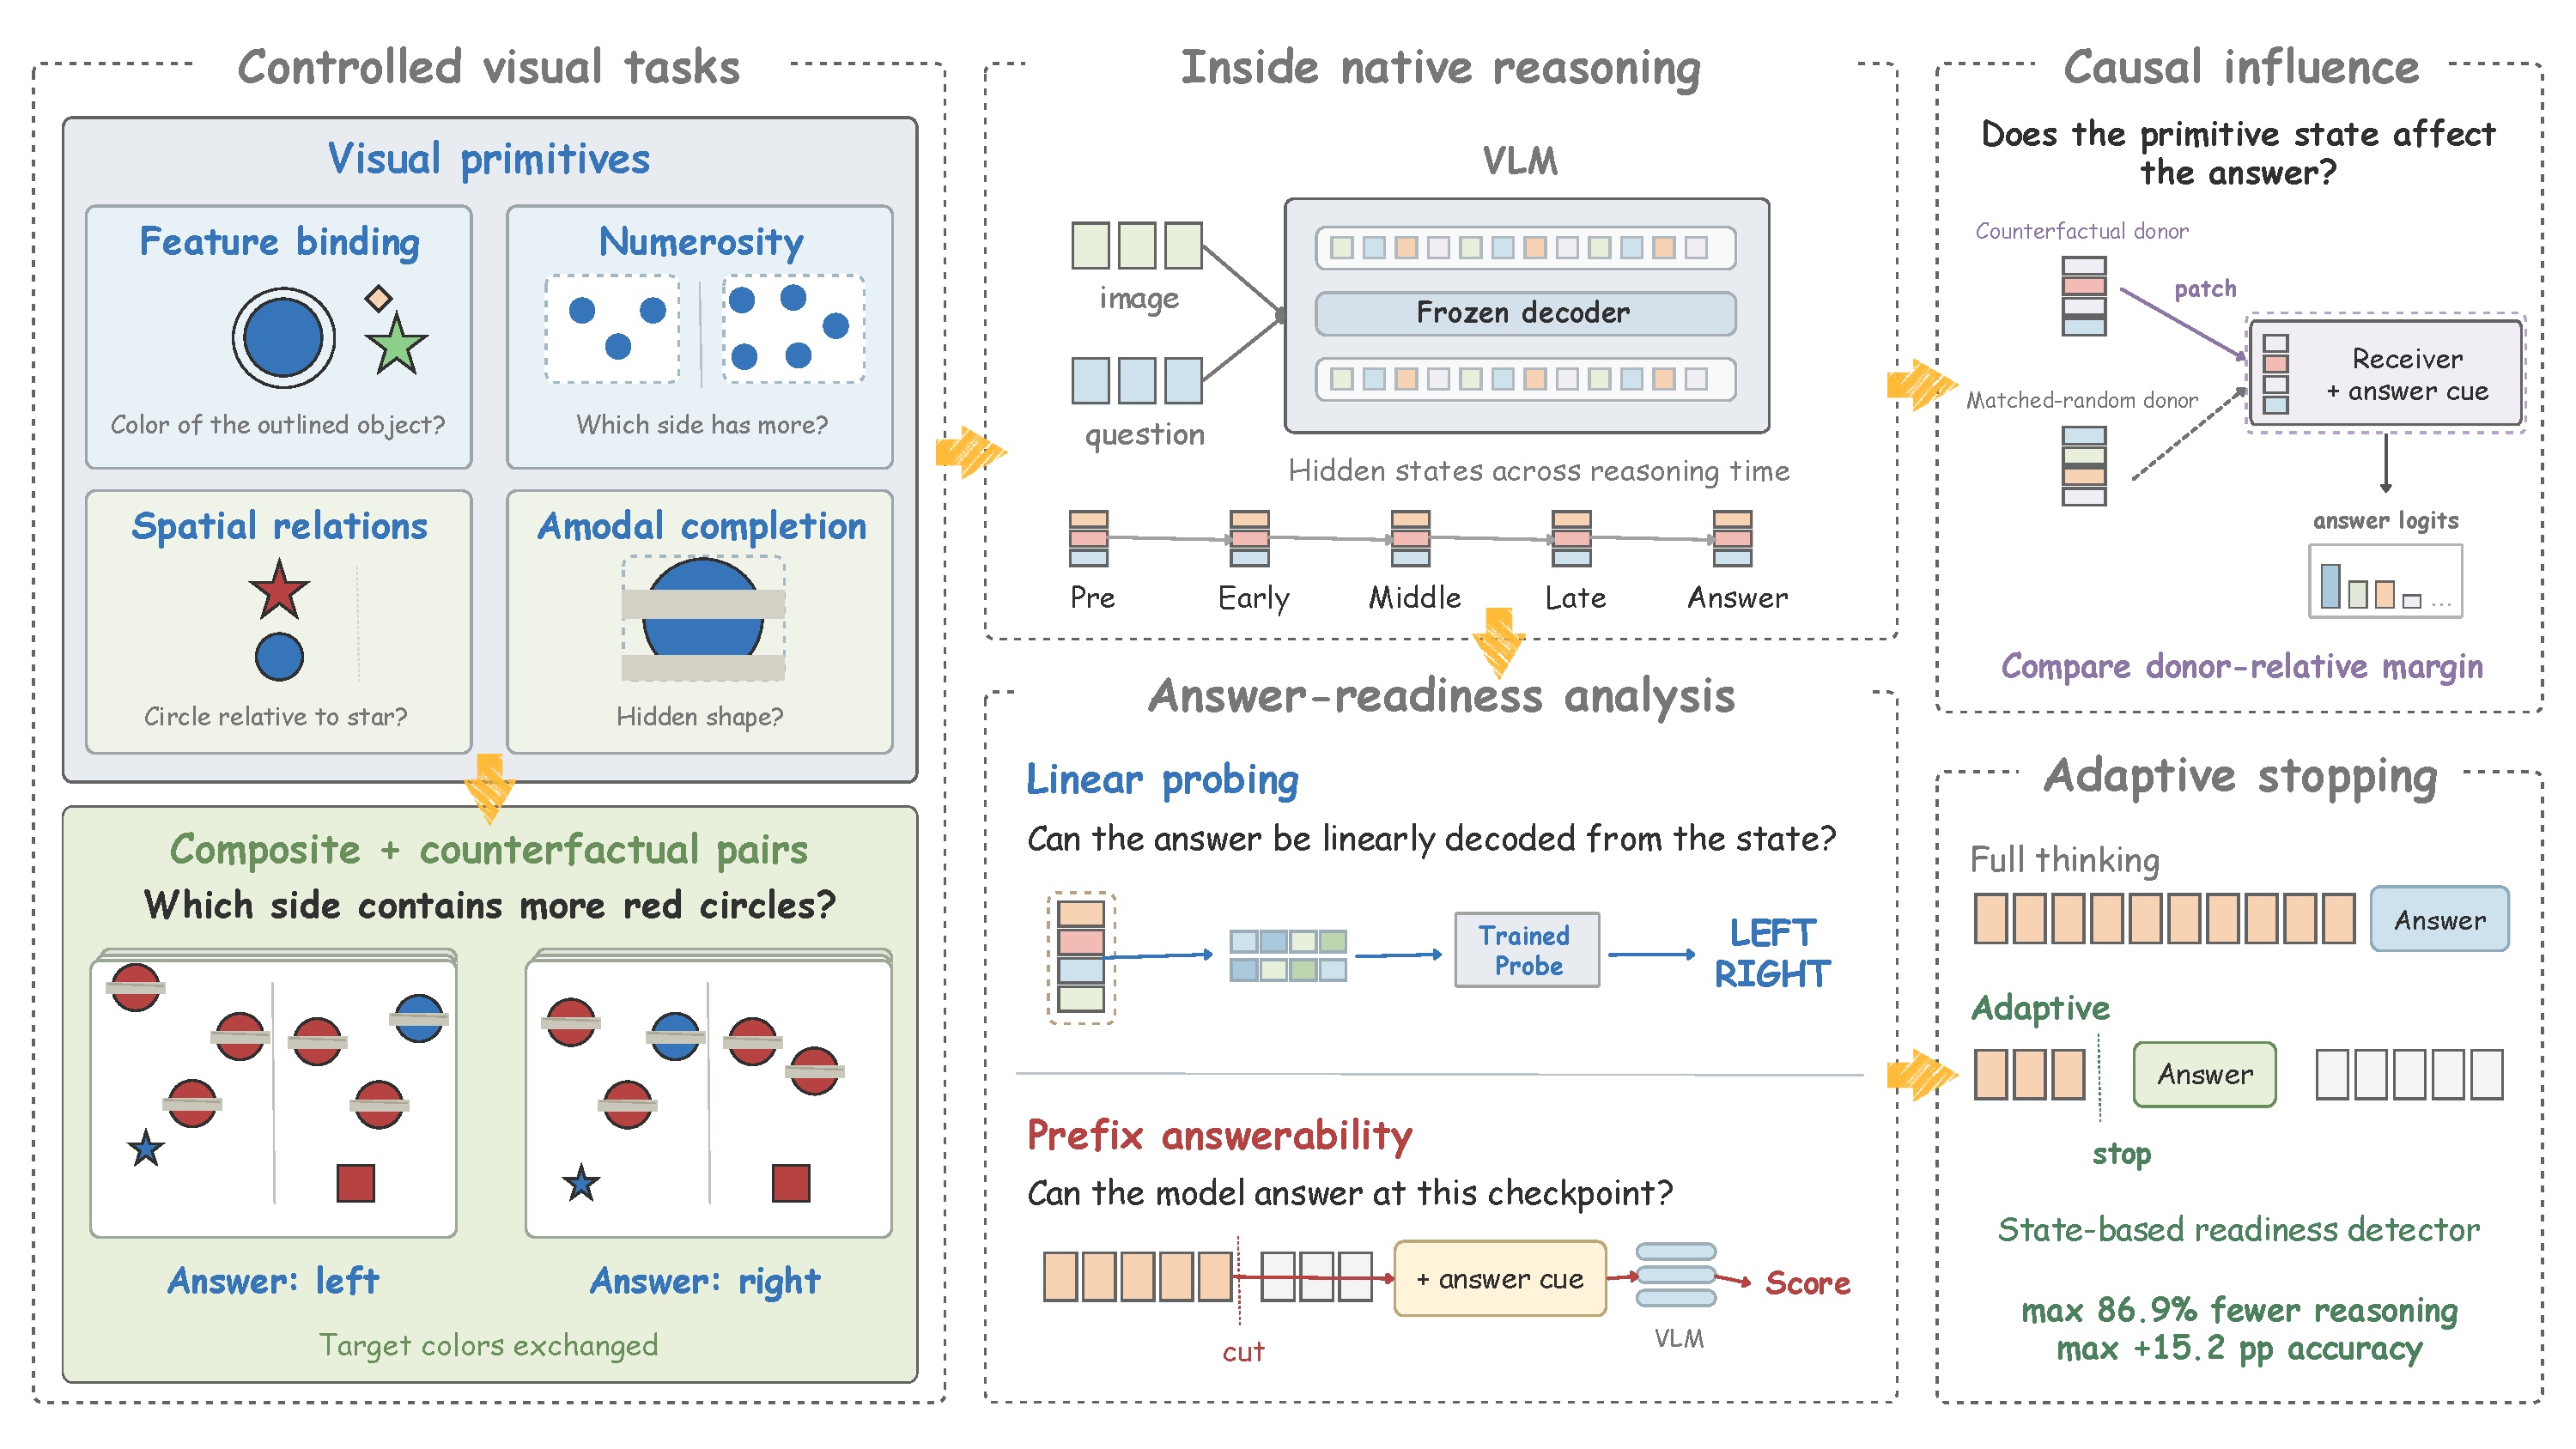
\includegraphics[width=\linewidth]{figures/paper_overview.pdf}
    \caption{Component visual judgments are available before reasoning starts, while the composite answer becomes available partway through the reasoning trace. Hidden-state probing, counterfactual interventions, and truncated-prefix evaluation locate where each judgment is resolved, and a readiness detector converts that point into an online stopping rule.}
    \label{fig:overview}
\end{figure}

\section{Related Work}

This section locates our contribution against three lines of work that each cover part of the interval we study, namely what visual evaluations report about the effect of reasoning, what mechanistic analyses recover from internal states, and how existing methods decide when reasoning should stop.

\paragraph{Multimodal reasoning and visual evaluation.}
Diagnostic benchmarks isolate compositional visual reasoning and cognitive abilities through controlled tasks \citep{johnson2017clevr,schiappa2024probing,huang2025visfactor}, while multimodal CoT methods develop reasoning procedures such as textual rationales and steps grounded in image regions or objects \citep{zhang2024multimodalcot,shao2024visualcot,li2025vocot}. Evaluations of reasoning quality, robustness, and efficiency show that additional thinking affects perception and reasoning tasks differently, and complementary analysis delineates which multimodal problems chain-of-thought reasoning can and cannot help with \citep{jiang2025mmecot,jin2026looklight}. These evaluations report what reasoning changes at the level of final answers, without showing where in the trace the change takes effect.

\paragraph{Interpreting visual representations in VLMs.}
Causal tracing and token interventions, developed for locating factual associations in language models \citep{meng2022locating}, have been adapted to locate visual information and examine its contribution to VLM predictions \citep{basu2024understanding,neo2025interpreting}. Information-flow studies identify task-dependent direct and text-mediated pathways alongside fallback behavior under intervention \citep{zhang2025crossmodal,salazar2026pathways}, and layer-wise probing separates visual grounding, semantic processing, and answer formatting \citep{yu2025multimodal}. These analyses operate within a single forward pass, so they locate where visual information resides without tracking how it is consumed as a reasoning trace unfolds.

\paragraph{Efficient reasoning and early exit.}
Hidden-state probes can predict eventual reasoning success or verify intermediate answers to support early exit \citep{afzal2025knowing,zhang2025reasoningmodels}, and trial-answer confidence or sufficiency assessment can decide when to stop \citep{yang2026deer,xiang2026thinking}. In VLMs, \citet{bi2026seeing} probe reasoning helpfulness and desired generation length, then control behavior through attention-head interventions. These criteria are defined on the text trace alone, and none is grounded in a measurement of when the visual answer itself becomes available.

Previous work treats the analysis of visual representations and the control of reasoning length as separate problems. We connect the two by measuring when a composite visual answer becomes available inside the trace and adopting that measurement as the stopping target, so the same quantity that explains how the answer forms decides when to produce it.
\section{Interpreting Composite Visual Reasoning}
\label{sec:interpretability}

This section examines how component visual judgments support the formation of a composite answer. We introduce the controlled tasks and counterfactual pairs, examine the behavioral performance, decodability, and causal role of the component judgments, and then trace how the Composite answer develops during reasoning.

\subsection{Interpretability Analysis Setup}
\label{sec:primitive}

The tasks below isolate the visual abilities that the Composite task later requires. Each one fixes a single answer-determining variable and holds the remaining scene content constant, so that behavioral and representational measurements can be attributed to that variable.

\paragraph{Feature Binding.}
Feature Binding associates visual attributes with the objects that carry them. Human illusory-conjunction errors show that features can be perceived yet incorrectly combined, which separates detecting an attribute from binding it to its source \citep{treisman1980feature,treisman1982illusory}. Each image contains multiple colored shapes, and one object is marked by a black outline. The model identifies the color of that object.

\paragraph{Numerosity.}
Numerosity concerns the quantities of non-symbolic sets, which infants discriminate before symbolic counting once continuous visual properties are controlled \citep{feigenson2004core,xu2000large}. The model compares dot arrays on opposite sides of a divider and selects the side containing more dots. We control the relationship between numerosity and total dot area, while the left/right answer format avoids requiring an exact numerical response.

\paragraph{Spatial Relations.}
Spatial Relations specify the position of a target relative to a reference object, and human judgments depend on attentional selection of the two objects whose relation is queried \citep{carlson1999what,logan1994spatial}. Black and gray outlines designate these two roles, respectively, while object colors and shapes vary across images. The model identifies whether the target is left, right, above, or below the reference.

\paragraph{Amodal Completion.}
Amodal Completion concerns perceiving a whole object from the visible portions of an occluded shape, where priming studies show that visible fragments can activate the completed interpretation \citep{kellman1991theory,sekuler1992perception}. We partially occlude a geometric shape and ask the model to identify the complete shape from candidate answers. It supplies the component judgment that the Composite task needs for partially hidden objects.

\paragraph{Composite Task.}
The Composite task asks which side of a divider contains more red circles among colored and partially occluded shapes. It combines shape recognition under occlusion, color--shape binding, left/right region assignment, and comparison of the resulting target counts, so it plays the role that ``challenge images'' play in primate vision, where the component judgments are individually easy but the joint solution emerges in the ventral stream only after an additional interval of recurrent processing \citep{kar2019evidence,kar2021fast}.


\paragraph{Counterfactual Pairs.}
For mechanistic comparisons, matched counterfactual pairs vary an answer-determining visual property while preserving the scene context \citep{gardner2020evaluating,bitton2021automatic}. Feature Binding, Numerosity, and Spatial Relations use separate single-image and intervention-pair datasets, while Amodal Completion and Composite are built as paired datasets. They supply matched contrasts and donor--receiver examples for state interventions, with one pair per task in Figure~\ref{fig:dataset_examples}. Construction, control conditions, and splits are in Appendix~\ref{app:data_generation}.

\subsection{Availability of Visual Primitives Without Reasoning}
\label{sec:answer_ready_states}

We first ask whether models possess the component visual abilities needed for the Composite task without generating explicit reasoning. Behavioral evaluation tests whether they can perform the individual judgments, layer-wise linear readouts test whether the corresponding variables are recoverable from internal representations, and counterfactual interventions test how those representations affect answering \citep{belinkov2021probing}.

\paragraph{Component judgments are available without reasoning.}
To test whether a reasoning trace is needed for the component judgments at all, we keep model parameters frozen, disable thinking, and ask each model to answer the four primitive tasks directly. Table~\ref{tab:primitive_behavior} shows that all four models exceed the task-specific guess levels, with higher performance on Feature Binding and Spatial Relations and more errors on Numerosity and Amodal Completion.

\begin{table}[t]
    \centering
    \small
    \footnotesize
    \setlength{\tabcolsep}{4.5pt}
    \caption{All four component judgments can be performed above the guess level without explicit reasoning. Answer accuracy (\%) on 1,000 images per task and model; guess is uniform random selection over the answer choices (two for Numerosity, four for the others).}
    \label{tab:primitive_behavior}
    \vspace{-1.5mm}
    \begin{tabular}{lccccc}
        \toprule
        Task
        & Qwen3.5-4B
        & Qwen3.5-9B
        & Gemma-4-E4B
        & Gemma-4-12B
        & Guess \\
        \midrule
        Feature Binding
        & 98.0
        & 99.8
        & 98.6
        & 99.9
        & 25.0 \\
        Numerosity
        & 79.6
        & 85.2
        & 72.4
        & 86.5
        & 50.0 \\
        Spatial Relations
        & 99.8
        & 100.0
        & 97.5
        & 89.5
        & 25.0 \\
        Amodal Completion
        & 76.8
        & 80.5
        & 81.4
        & 72.9
        & 25.0 \\
        \midrule
        \textbf{Avg}
        & \textbf{88.6}
        & \textbf{91.4}
        & \textbf{87.5}
        & \textbf{87.2}
        & 31.3 \\
        \bottomrule
    \end{tabular}
\end{table}



\paragraph{Primitive variables are linearly recoverable across depth.}
Behavioral success shows that the judgments are available, without showing where the corresponding information resides. To locate it, we mean-pool image-token hidden states at each layer:
\begin{equation}
    v_i^{(\ell)}=\frac{1}{|\mathcal I_i|}
    \sum_{t\in\mathcal I_i}h_{i,t}^{(\ell)},
\end{equation}
where $h_{i,t}^{(\ell)}$ is the representation of sample $i$ at layer $\ell$ and token position $t$, and $\mathcal I_i$ contains its image-token positions. We standardize these vectors using training-set statistics to obtain $z_i^{(\ell)}$, whose rows form the training matrix $Z_\ell$. For each model and task, we fit an independent ridge linear readout at every layer, keeping the VLM frozen and fitting only the readout matrix:
\begin{equation}
    W_\ell^*=\arg\min_W\|Z_\ell W-Y\|_F^2+\lambda\|W\|_F^2,
    \qquad
    f_{\mathrm{read}}\bigl(z_i^{(\ell)}\bigr)=\arg\max_c\bigl(z_i^{(\ell)}W_\ell^*\bigr)_c.
\end{equation}
Here $Y$ contains one-hot semantic labels, which are the target color, the more numerous side, the spatial direction, or the complete shape depending on the task, $\lambda$ controls regularization, and $f_{\mathrm{read}}$ denotes the resulting readout. Because the only fitted parameters are those of $f_{\mathrm{read}}$, its accuracy reflects what the frozen states already carry.

We evaluate each readout on held-out samples, keeping both members of a pair in the same split. To distinguish visual information from cues in the question, we independently fit the same readout on mean-pooled question-token states from inputs without an image. The readout predicts a semantic label directly, so for Amodal Completion it selects one of six complete shapes while behavioral evaluation selects among the four candidates shown in the question. Label spaces, split sizes, and fitting details appear in Appendix~\ref{app:primitive_analysis}.

The upper row of Figure~\ref{fig:primitive_analysis} shows that the visual variables are linearly recoverable across multiple depths, with task- and model-dependent profiles. Numerosity and complete-shape readouts achieve high accuracy, while Feature Binding and Spatial Relations vary more with depth. Question-only controls sit near the guess level for the first three tasks, and rise above it for Amodal Completion because the varying candidate list carries partial information about the shape label. Image-conditioned readouts exceed this control through most layers, indicating recoverable visual information in the states. We next test how replacing these states affects answering.

\paragraph{Recoverable states also drive the answer, but only at some depths.}
Decodability shows that a variable is present in the states, without showing that the model uses it. To test whether these states carry the information the answer depends on, we replace them across counterfactual pairs. For each pair, we treat one sample as the receiver and the other, whose correct answer differs, as the donor. At the input to a selected decoder block, we replace the receiver's image-token states with the corresponding donor states and resume the forward pass:
\begin{equation}
    f_{\mathrm{patch}}(r,d,\ell)\quad\text{assigns}\quad
    H_{r,\mathcal I_r}^{(\ell)}\leftarrow H_{d,\mathcal I_d}^{(\ell)}.
\end{equation}
Whereas $f_{\mathrm{read}}$ asks what the states carry, $f_{\mathrm{patch}}$ asks what they control. We intervene in both directions and retain pairs for which both original answers are correct under the intervention scoring protocol, which makes the retained set small and model-dependent. A matched-random donor comes from another pair with the receiver's semantic label and supplies states at the same token region. Parameters stay frozen and patching needs no training.

Logit differences capture partial effects of activation patching even when the predicted answer does not change \citep{heimersheim2024activation}. We use the donor-relative margin $m=s(y_d)-s(y_r)$, where $s(y)$ is the candidate answer logit score and $y_d$ and $y_r$ are the donor and receiver answers. To summarize how consistently interventions move the scores toward the donor, we report the difference between the proportions of targeted and matched-random replacements that increase this margin over the unpatched receiver:
\begin{equation}
    \Delta_{\mathrm{patch}}=100\left[
    \Pr(m_{\mathrm{target}}>m_{\mathrm{base}})
    -\Pr(m_{\mathrm{random}}>m_{\mathrm{base}})
    \right].
\end{equation}
Here $m_{\mathrm{base}}$ is the unpatched receiver margin, so positive $\Delta_{\mathrm{patch}}$ means counterfactual replacement increases the donor-relative margin more often than the control. This percentage-point difference measures the frequency of directional effects, not their magnitude or the rate of answer flips. Answer scoring and matching criteria appear in Appendix~\ref{app:primitive_analysis}.

\begin{figure}[t]
    \centering

\includegraphics[width=0.68\textwidth]{figures/primitive_decodability_legend.png}
    \par\vspace{-2pt}

    \begin{subfigure}[t]{0.245\textwidth}
        \centering
        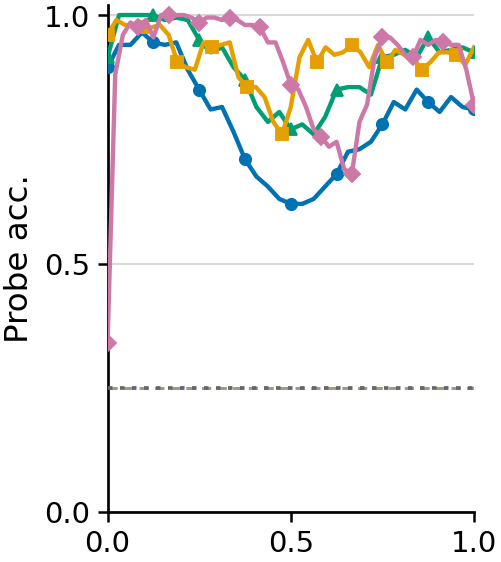
\includegraphics[width=\linewidth]{figures/primitive_decodability_feature_binding.png}
        \caption{\scriptsize Feature Binding}
    \end{subfigure}\hfill
    \begin{subfigure}[t]{0.245\textwidth}
        \centering
        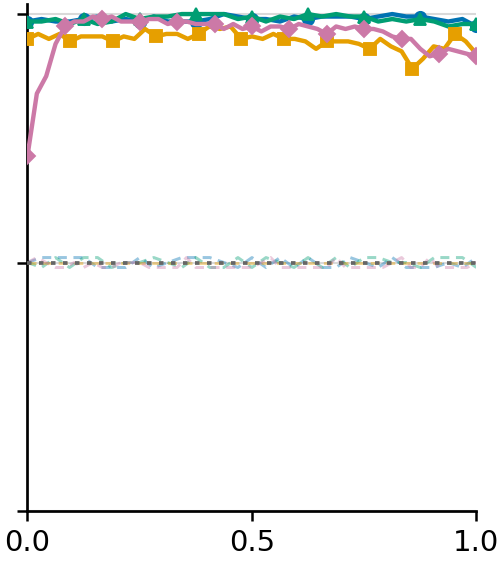
\includegraphics[width=\linewidth]{figures/primitive_decodability_numerosity.png}
        \caption{\scriptsize Numerosity}
    \end{subfigure}\hfill
    \begin{subfigure}[t]{0.245\textwidth}
        \centering
        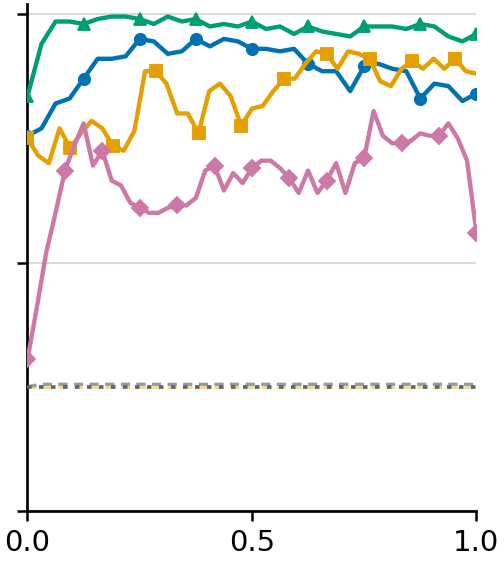
\includegraphics[width=\linewidth]{figures/primitive_decodability_spatial_relations.png}
        \caption{\scriptsize Spatial Relations}
    \end{subfigure}\hfill
    \begin{subfigure}[t]{0.245\textwidth}
        \centering
        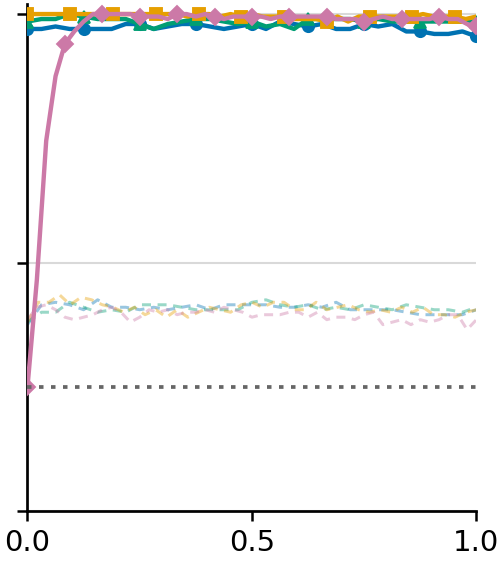
\includegraphics[width=\linewidth]{figures/primitive_decodability_amodal_completion.png}
        \caption{\scriptsize Amodal Completion}
    \end{subfigure}

    \par\vspace{2pt}


\includegraphics[width=0.56\textwidth]{figures/primitive_causal_legend.png}
    \par\vspace{-2pt}

    \begin{subfigure}[t]{0.245\textwidth}
        \centering
        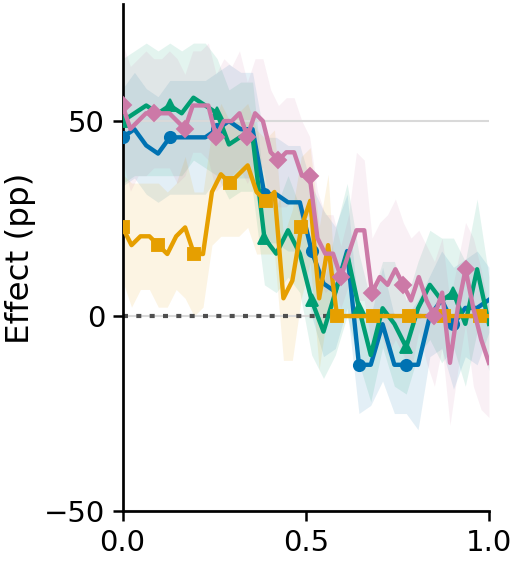
\includegraphics[width=\linewidth]{figures/primitive_causal_feature_binding.png}
        \caption{\scriptsize Feature Binding}
    \end{subfigure}\hfill
    \begin{subfigure}[t]{0.245\textwidth}
        \centering
        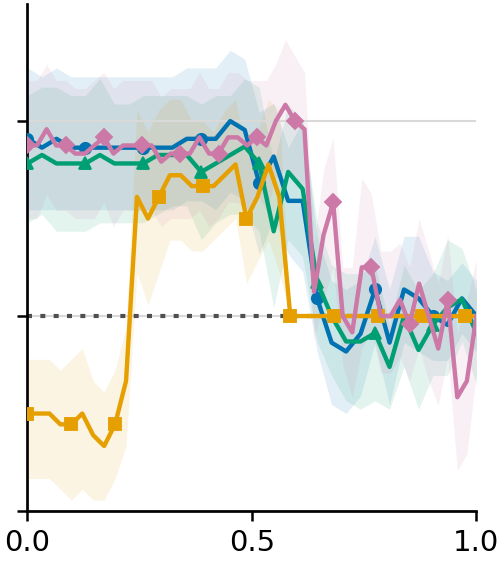
\includegraphics[width=\linewidth]{figures/primitive_causal_numerosity.png}
        \caption{\scriptsize Numerosity}
    \end{subfigure}\hfill
    \begin{subfigure}[t]{0.245\textwidth}
        \centering
        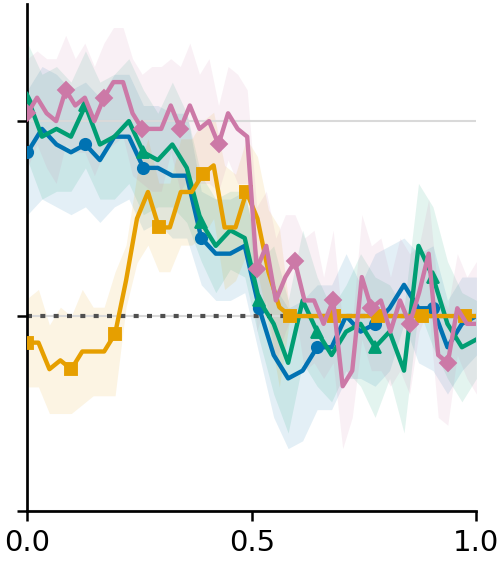
\includegraphics[width=\linewidth]{figures/primitive_causal_spatial_relations.png}
        \caption{\scriptsize Spatial Relations}
    \end{subfigure}\hfill
    \begin{subfigure}[t]{0.245\textwidth}
        \centering
        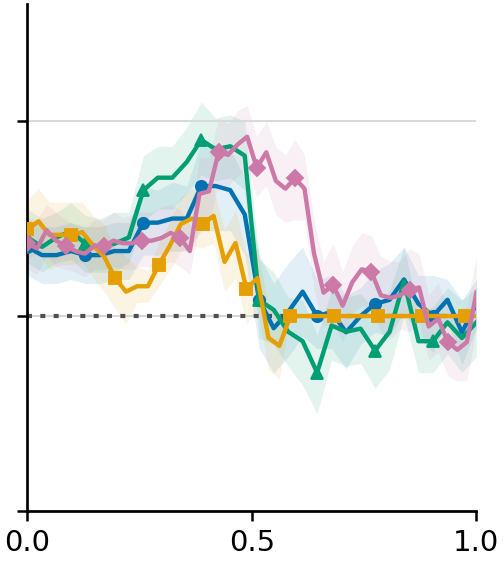
\includegraphics[width=\linewidth]{figures/primitive_causal_amodal_completion.png}
        \caption{\scriptsize Amodal Completion}
    \end{subfigure}

    \caption{Every controlled visual variable stays decodable across most of the depth, while its causal influence on the answer is concentrated in early-to-middle layers. Upper row: held-out readout accuracy (solid: image-conditioned; dashed: question-only; dotted gray: task-specific guess). Lower row: percentage-point difference between task-targeted and matched-random moves-toward-donor rates in the image-token region, with paired-bootstrap 95\% CIs. Normalized layer depth divides the layer index by the largest tested index.}
    \label{fig:primitive_analysis}
\end{figure}

The lower row of Figure~\ref{fig:primitive_analysis} shows that targeted patching shifts scores toward the donor more consistently relative to the control in early-to-middle layers than at the final tested block. Reading the two rows together exposes a dissociation, because a variable stays linearly recoverable at depths where replacing it no longer moves the answer, so decodability marks where information survives and patching marks where it is still being consumed. Two consequences follow. The component judgments are not the bottleneck, since each one is both present and causally live within a single forward pass, which places the difficulty of the Composite task in integrating these judgments and not in perceiving them. A probe that recovers a variable also cannot certify that the model acts on it, which is why the analysis that follows measures readiness by forcing an answer from a truncated prefix and why the stopping rule of Section~\ref{sec:early_stopping} is supervised by forced-answer correctness.

\subsection{Development of Composite Answer Readiness}

We now examine how native thinking supports a Composite decision and when the accumulated reasoning becomes sufficient to answer.

\paragraph{Reasoning improves counterfactual consistency.}
To measure what explicit reasoning contributes once the component judgments must be used jointly, we compare no-thinking and native-thinking responses on the same held-out pairs. Sample accuracy scores individual images, while pair-consistent accuracy requires both counterfactual members to be correct.

\begin{table}[t]
    \centering
    \scriptsize
    \renewcommand{\arraystretch}{0.95}
    \setlength{\tabcolsep}{2pt}
    \caption{Native thinking improves counterfactual consistency. Values are accuracy (\%) with pair-bootstrap 95\% CIs; $\Delta$ is the reasoning-induced change in percentage points; budget hit counts thinking-mode runs (of 200) that reach the generation limit.}
    \label{tab:thinking_behavior}
    \vspace{-1.5mm}
    \begin{tabular*}{\textwidth}{
        @{\extracolsep{\fill}}
        l
        ccc
        ccc
        c@{}
    }
        \toprule
        & \multicolumn{3}{c}{\textbf{Sample Accuracy}}
        & \multicolumn{3}{c}{\textbf{Pair-Consistent Accuracy}} & \textbf{Budget hit} \\
        \cmidrule(lr){2-4}
        \cmidrule(lr){5-7}\cmidrule(lr){8-8}
        Model
        & Non-thinking
        & \textbf{Thinking}
        & $\Delta$
        & Non-thinking
        & \textbf{Thinking}
        & $\Delta$ & Count (\%) \\
        \midrule

        Qwen3.5-4B
        & \makecell{58.5\\{\scriptsize [53.0,64.0]}}
        & 
          \makecell{\textbf{80.0}\\{\scriptsize [74.0,86.0]}}
        & $\uparrow\,21.5$
        & \makecell{26.0\\{\scriptsize [18.0,35.0]}}
        & 
          \makecell{\textbf{67.0}\\{\scriptsize [58.0,76.0]}}
        & $\uparrow\,41.0$ & 38 (19.0\%) \\

        Qwen3.5-9B
        & \makecell{66.5\\{\scriptsize [61.5,71.5]}}
        & 
          \makecell{\textbf{94.0}\\{\scriptsize [90.5,97.0]}}
        & $\uparrow\,27.5$
        & \makecell{36.0\\{\scriptsize [27.0,45.0]}}
        & 
          \makecell{\textbf{89.0}\\{\scriptsize [83.0,95.0]}}
        & $\uparrow\,53.0$ & 11 (5.5\%) \\

        Gemma-4-E4B
        & \makecell{52.0\\{\scriptsize [49.0,55.0]}}
        & 
          \makecell{\textbf{73.5}\\{\scriptsize [67.0,80.0]}}
        & $\uparrow\,21.5$
        & \makecell{7.0\\{\scriptsize [2.0,12.0]}}
        & 
          \makecell{\textbf{57.0}\\{\scriptsize [47.0,67.0]}}
        & $\uparrow\,50.0$ & 0 (0.0\%) \\

        Gemma-4-12B
        & \makecell{\textbf{57.5}\\{\scriptsize [54.0,61.0]}}
        & 
          \makecell{54.5\\{\scriptsize [47.0,62.0]}}
        & $\downarrow\,3.0$
        & \makecell{15.0\\{\scriptsize [8.0,22.0]}}
        & 
          \makecell{\textbf{34.0}\\{\scriptsize [25.0,43.0]}}
        & $\uparrow\,19.0$ & 84 (42.0\%) \\

        \midrule
        \textbf{Avg}
        & 58.6
        & \textbf{75.5}
        & $\uparrow\,16.9$
        & 21.0
        & \textbf{61.8}
        & $\uparrow\,40.8$ & 133 (16.6\%) \\

        \bottomrule
    \end{tabular*}
\end{table}

Table~\ref{tab:thinking_behavior} shows that native thinking improves pair-consistent accuracy across all four models. Sample accuracy also improves for three models, while Gemma-4-12B declines despite its higher pair consistency. This model also frequently reaches the generation limit, although the comparison does not isolate budget exhaustion as the cause of its lower sample accuracy. These final-response results leave open a temporal question. Does the model accumulate enough information to answer before it finishes its full reasoning trace?

\paragraph{Tracing when the Composite answer becomes available.}
Final-response accuracy reports whether reasoning helped, without locating the point at which it did. To recover that point, we follow native traces at five checkpoints spanning the trace, from before reasoning (\textsc{Pre}) through its early and middle stages to the last reasoning token (\textsc{Late}) and the position before the final choice token (\textsc{Answer}). For each model, validation pairs select a layer using pre-reasoning answer decodability, and that layer stays fixed across checkpoints and test samples. Trajectory analysis retains pairs whose two traces provide usable checkpoints and a parsed answer, so its sample counts can differ from the behavioral evaluation. Positions, selected layers, and split construction appear in Appendix~\ref{app:reasoning_checkpoints} and Appendix~\ref{app:data_generation}.

At each checkpoint, we fit an independent ridge linear readout to the hidden state at the selected layer and token position, targeting the correct Composite answer, left or right. The VLM remains frozen, and only the readout is fitted using the standardized features and ridge objective of Section~\ref{sec:answer_ready_states}, trained and tested on states from the same pair-preserving splits. Its held-out accuracy measures whether the correct answer can be recovered from that state.

To measure whether the accumulated prefix supports answering, we truncate each trace at the checkpoint, append a fixed answer suffix, and score the two candidate answers with the frozen model:
\begin{equation}
    f_{\mathrm{force}}(i,t)
    =\arg\max_{c\in\{\mathrm{left},\mathrm{right}\}}
    s_\theta(c\mid x_i,r_{i,\leq t},a),
    \qquad
    U(t)=\frac{1}{N}\sum_{i=1}^{N}
    \mathbf{1}\bigl[f_{\mathrm{force}}(i,t)=y_i\bigr].
\end{equation}
Here $x_i$ is the image and prompt, $r_{i,\leq t}$ is the prefix through checkpoint $t$, $a$ is the fixed answer suffix that specifies the format without supplying the answer, and $s_\theta$ is the candidate logit score. We operationalize answer readiness through this prefix-conditioned accuracy. While $f_{\mathrm{read}}$ reads a single hidden state, $f_{\mathrm{force}}$ answers from the complete retained prefix, including any verbalized intermediate results. Computing it requires a reference answer, available in this analysis but not at inference time.

\begin{figure}[t]
    \centering
    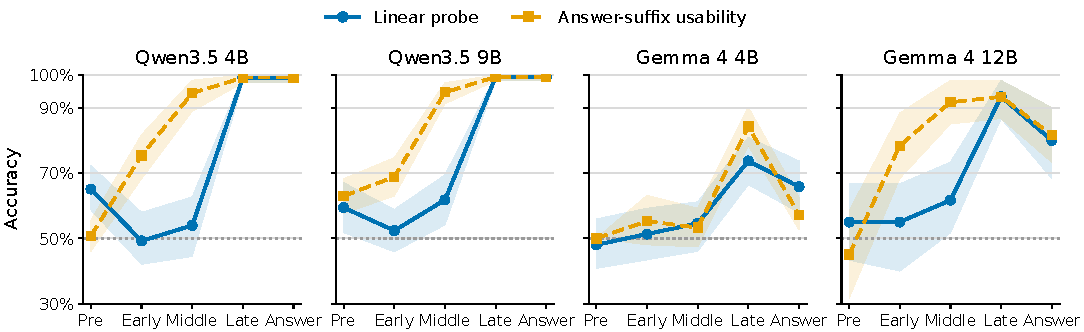
\includegraphics[width=\linewidth]{figures/answer_state_dynamics.pdf}
    \caption{The Composite answer is not ready before reasoning starts, and becomes both decodable and directly answerable as the trace unfolds. Each panel follows one model through five reasoning checkpoints; blue: probe accuracy for the final Composite answer from a fixed-depth hidden state; orange: accuracy after truncating the native trace at that checkpoint and appending a fixed answer suffix. Shaded: pair-bootstrap 95\% CIs; dotted: binary guess.}
    \label{fig:answer_state_dynamics}
\end{figure}

\paragraph{Answer readiness develops during native thinking.}
Figure~\ref{fig:answer_state_dynamics} shows that answer decodability and prefix-conditioned answering are not consistently high across models before reasoning. Both improve as reasoning proceeds but at different rates, with prefix-conditioned accuracy rising earlier for the Qwen models and Gemma-4-12B and later for Gemma-4-E4B, and by \textsc{Late} both are high across all four models. The Composite answer therefore becomes both more recoverable from hidden states and more accessible through prefix-conditioned answering during native reasoning.

Moving from the last reasoning token (\textsc{Late}) to the position before the final choice (\textsc{Answer}) does not uniformly improve either measurement, since both Qwen models retain high performance while both Gemma models decline. Readiness is therefore reached inside the trace and not at its end, so the tokens generated after that point are spent on an answer the state already supports. Table~\ref{tab:thinking_behavior} prices them, since 16.6\% of thinking runs on average exhaust the generation budget without ever committing to an answer. A quantity the analysis reads offline can also be read online, which raises the question addressed next. Can the evolving hidden state identify when to transition from reasoning to answering?

\section{Answer-Readiness-Guided Early Stopping}
\label{sec:early_stopping}

The goal of this section is to convert the preceding analysis into a saving at inference time. Section~\ref{sec:interpretability} supplies both halves of the trade. Unfolding the computation in time is what makes the composite judgment solvable, matching the visual computations that the primate ventral stream resolves only through additional recurrent processing \citep{lamme2000distinct,kar2019evidence}, and the prefix-conditioned measurements show that this unfolding finishes its work before the trace does, which leaves the remaining tokens as cost without benefit. We therefore read answer readiness online with a lightweight detector, trained separately for each model and dataset at the layers selected on Composite. This decision has a precedent in human perceptual decision-making, where an evolving centro-parietal signal accumulates with decision evidence and reaches a stereotyped amplitude just before commitment, independently of sensory modality and motor response \citep{oconnell2012supramodal}. Our detector $f_{\mathrm{ready}}$ is a functional analogue of that signal, reading the current state together with its change since the preceding checkpoint, so $\eta$ acts as an operational decision bound instead of a tuned constant.

\paragraph{Reference-free readiness from state dynamics.}
Our detector replaces the reference answer that $f_{\mathrm{force}}$ needs with a prediction made from the state itself. We truncate native traces at regular checkpoints, insert a fixed final-answer transition, and label each checkpoint by whether the frozen model's resulting answer is correct. A state alone does not indicate how quickly readiness is approaching, so the detector reads the current state together with its change since the preceding checkpoint and the elapsed reasoning length:
\begin{equation}
    f_{\mathrm{state}}(t)=\bigl[h_t^{(\ell)},\ d_t^{(\ell)},\ t/B\bigr],
    \qquad
    f_{\mathrm{ready}}(t)=\sigma\bigl(w^\top\tilde f_{\mathrm{state}}(t)+b\bigr),
\end{equation}
where $d_t^{(\ell)}$ is the change from the preceding checkpoint state, using a zero reference at the first checkpoint. The tilde denotes training-set standardization, and $B$ is the generation budget. We freeze the VLM and fit only $w$ and $b$ with class-weighted binary cross-entropy, so $f_{\mathrm{ready}}$ adds one linear readout over states the model already computes. Its target is correctness under immediate answering, which makes it an online estimate of the quantity that $f_{\mathrm{force}}$ measures offline.

\paragraph{Stopping at a validated decision bound.}
Every $\Delta$ reasoning tokens, the detector checks whether $f_{\mathrm{ready}}(t)\geq\eta$ and triggers the same final-answer transition at the first crossing. Neither the interval $\Delta$ nor the bound $\eta$ is fixed by hand. Validation selects $\eta$ to minimize reasoning length within an accuracy-loss tolerance relative to full thinking, so each model and dataset receives the bound its own readiness trajectory supports. Without a crossing, generation continues to natural termination or the budget limit.

\section{Experiments}
\label{sec:experiments}

The goal of this section is to test whether readiness read online supports the same decision the offline analysis licensed, which requires the stopping rule to preserve answer quality while removing the reasoning that follows readiness. Each model is compared against its own full-thinking generation under an identical budget and extraction rule, so differences reflect the stopping decision alone.

\subsection{Experimental Setup}

The two benchmarks vary the factors a stopping rule has to survive, since MMStar \citep{chen2024we} spans coarse and fine-grained perception, science, and mathematics under a fixed multiple-choice format, while RealWorldQA \citep{xai2024realworldqa} uses real-world photographs and mixes multiple-choice with open short-answer questions. We evaluate 1,500 MMStar and 765 RealWorldQA questions using two-fold cross-validation, training and validating on one fold and testing on the other, with checkpoints from each question and duplicate RealWorldQA images kept together so each question contributes one held-out prediction per condition. We set the checkpoint interval to $\Delta=256$ tokens, give full thinking and adaptive stopping the same budget $B=6{,}144$ tokens, and compare final-answer accuracy and mean reasoning tokens under a common protocol. Training, splits, and scoring are detailed in Appendix~\ref{app:early_stopping}.

\subsection{Main Results}

\paragraph{Accuracy is preserved under aggressive length reduction.}
Adaptive stopping reduces reasoning length for every model while raising average accuracy (upper block of Table~\ref{tab:early_stopping_main}), with the largest gain on Gemma-4-12B, and total output length also decreases so the savings extend beyond the reasoning segment. Part of the gain arises because $f_{\mathrm{ready}}$ reads hidden states instead of generated text, which lets it trigger the answer transition on traces the model would not have closed on its own. Per-fold results appear in Appendix~\ref{app:early_stopping_realworldqa}.

\paragraph{The stopping rule holds when the answer space is not a fixed candidate list.}
The lower block of Table~\ref{tab:early_stopping_main} extends this comparison to a dataset containing both multiple-choice and short-answer questions. All four models use fewer reasoning tokens and average accuracy improves, with a small decrease on Gemma-4-E4B, so the length reductions carry over to answers not drawn from a fixed candidate set while the accuracy benefit depends on the model. One rule, instantiated per model and dataset at layers selected on the controlled Composite task, therefore transfers to two benchmarks with different answer formats, which indicates that answer readiness is a property of the reasoning process and not of a question format. Stopping also reshapes the output, since the recovered answers come from two sources and the checkpoints at which the detector fires differ by model instead of following a common truncation length (Appendix~\ref{app:completion_analysis} and Appendix~\ref{app:stopping_behavior}).

\begin{table}[t]
    \centering
    \scriptsize
    \renewcommand{\arraystretch}{0.95}
    \setlength{\tabcolsep}{2pt}
    \caption{Adaptive stopping cuts reasoning cost on both benchmarks while raising average accuracy. All held-out cases per model (1,500 MMStar and 765 RealWorldQA); accuracy in \%, reasoning tokens as means, $\Delta$ in percentage points, reduction as the token decrease.}
    \label{tab:early_stopping_main}
    \vspace{-1.5mm}
    \begin{tabular*}{\textwidth}{
        @{\extracolsep{\fill}}
        ll
        ccc
        ccc@{}
    }
        \toprule
        & &  \multicolumn{3}{c}{\textbf{Accuracy (\%)}}
        & \multicolumn{3}{c}{\textbf{Reasoning Tokens}} \\
        \cmidrule(lr){3-5}
        \cmidrule(lr){6-8}
        Benchmark
        & Model
        & Full
        & \textbf{Stop}
        & $\Delta$
        & Full
        & \textbf{Stop}
        & Reduction \\
        \midrule
        \multirow{5}{*}{MMStar}
        & Qwen3.5-4B & 60.87 & \textbf{67.47} & $\uparrow\,6.60$ & 2,041 & \textbf{469} & $77.0\%$ \\
        
        & Qwen3.5-9B & 63.27 & \textbf{67.93} & $\uparrow\,4.66$ & 1,951 & \textbf{256} & $86.9\%$ \\
        
        & Gemma-4-E4B & 52.33 & \textbf{54.47} & $\uparrow\,2.14$ & 753 & \textbf{439} & $41.7\%$ \\
        
        & Gemma-4-12B & 46.67 & \textbf{61.87} & $\uparrow\,15.20$ & 1,854 & \textbf{246} & $86.7\%$ \\
        \cmidrule(l){2-8}
        & \textbf{Avg} & 55.79 & \textbf{62.94} & $\uparrow\,7.15$ & 1,650 & \textbf{353} & $\mathbf{78.6\%}$ \\
        \midrule
        \multirow{5}{*}{RealWorldQA}
        & Qwen3.5-4B & 72.81 & \textbf{75.42} & $\uparrow\,2.61$ & 1,696 & \textbf{285} & $83.2\%$ \\
        
        & Qwen3.5-9B & 72.94 & \textbf{77.91} & $\uparrow\,4.97$ & 1,606 & \textbf{248} & $84.6\%$ \\
        
        & Gemma-4-E4B & \textbf{58.17} & 57.12 & $\downarrow\,1.05$ & 442 & \textbf{346} & $21.8\%$ \\
        
        & Gemma-4-12B & 60.13 & \textbf{66.80} & $\uparrow\,6.67$ & 859 & \textbf{293} & $65.9\%$ \\
        \cmidrule(l){2-8}
        & \textbf{Avg} & 66.01 & \textbf{69.31} & $\uparrow\,3.30$ & 1,151 & \textbf{293} & $\mathbf{74.5\%}$ \\
        \bottomrule
    \end{tabular*}
\end{table}

\vspace{-4mm}
\section{Conclusion}\label{sec:conclusion}
\vspace{-1mm}

We studied how visual judgments support composite answers in VLMs. Component abilities are available without explicit reasoning, while composite decodability and prefix-conditioned answering develop during native thinking, so a prefix supports a correct answer before termination. A lightweight detector converts this into early stopping that shortens reasoning on MMStar and RealWorldQA while improving accuracy, with part of the gain from traces full thinking never closes.

\bibliography{main2}
\bibliographystyle{iclr2027_conference}

\appendix
\section{Datasets and Mechanistic Analysis}
\label{app:data_generation}

Table~\ref{tab:dataset_splits} summarizes the synthetic datasets and their analysis splits.

\begin{figure}[H]
    \centering
    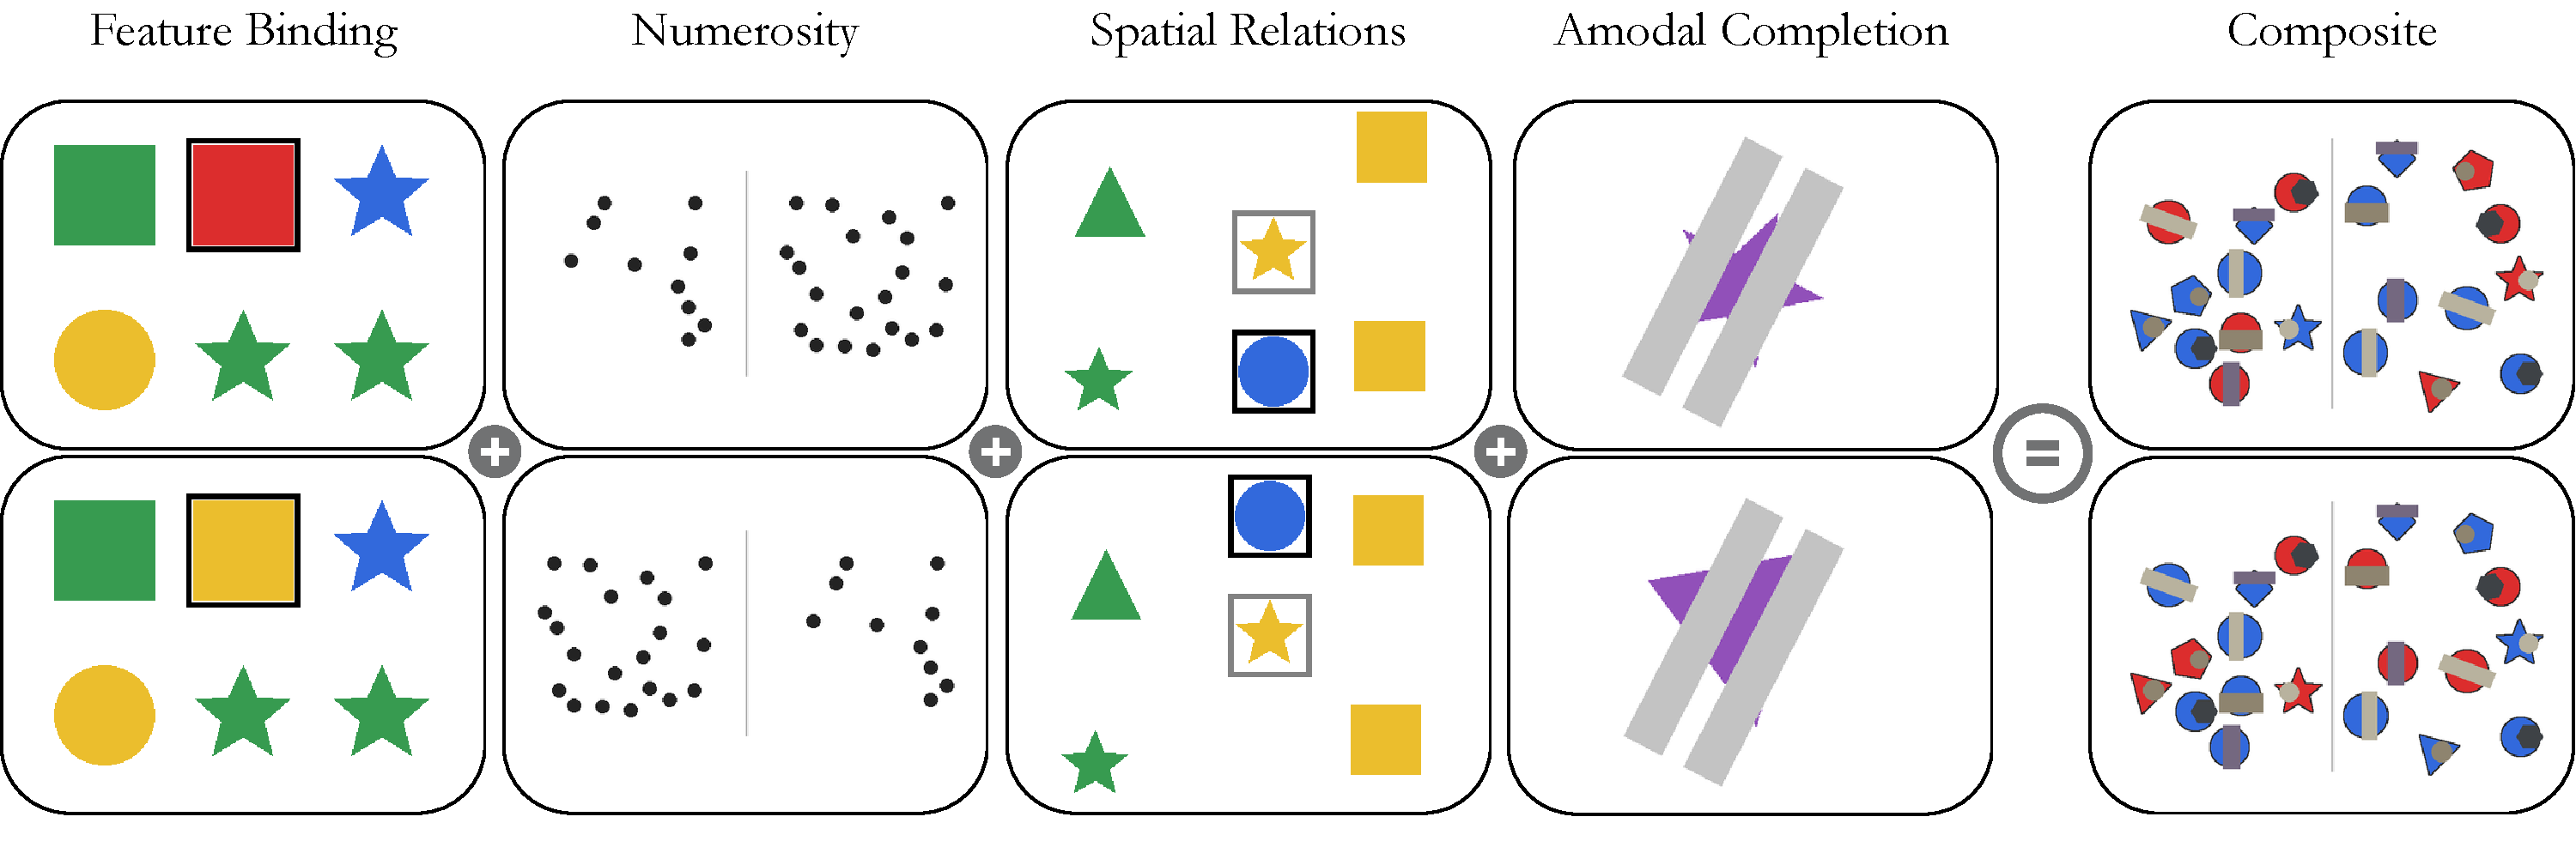
\includegraphics[width=0.92\textwidth]{figures/Controlled visual tasks.pdf}
    \caption{\textbf{Each controlled task isolates one answer-determining visual variable.} Every column shows a counterfactual pair in which the task-relevant variable and the correct answer change together while the remaining scene content is preserved.}
    \label{fig:dataset_examples}
\end{figure}


\begin{table}[H]
    \centering
    \small
    \renewcommand{\arraystretch}{1.05}
    \setlength{\tabcolsep}{2pt}
    \caption{\textbf{Synthetic dataset sizes and analysis splits.} Counts are images. Primitive splits are used for linear probing, and the Composite split is used for reasoning-trajectory analysis before trace filtering. Behavioral evaluation uses all 1,000 images per primitive and the 200-image Composite test set. Paired images remain in the same split.}
    \label{tab:dataset_splits}
    \begin{tabular*}{\textwidth}{@{\extracolsep{\fill}}lcccccc@{}}
        \toprule
        & & & \multicolumn{3}{c}{\textbf{Analysis Split}} & \\
        \cmidrule(lr){4-6}
        Dataset & Images & Choices & Train & Validation & Test & Split Unit \\
        \midrule
        Feature Binding & 1,000 & 4 & 800 & -- & 200 & Image \\
        Numerosity & 1,000 & 2 & 800 & -- & 200 & Image \\
        Spatial Relations & 1,000 & 4 & 800 & -- & 200 & Image \\
        Amodal Completion & 1,000 & 4 & 800 & -- & 200 & Pair \\
        Composite & 1,000 & 2 & 640 & 160 & 200 & Pair \\
        \bottomrule
    \end{tabular*}
\end{table}


\subsection{Primitive Dataset Construction}

Each primitive dataset is rendered procedurally so that the answer-determining variable varies independently of the remaining scene content. The paragraphs below give the generation parameters for each task.

\paragraph{Feature Binding.}
Feature Binding uses four target colors (red, blue, green, and yellow), four shapes, 4--8 objects per image, and three layout templates. Target shape, size, and position also vary.

\paragraph{Numerosity.}
Numerosity crosses three larger-to-smaller count ratios (2.0, 1.5, and 1.25) with three total-dot-area conditions, which are congruent with numerosity, approximately matched between sides, and incongruent. Dot positions are sampled within fixed regions without overlap, and the more numerous side is balanced.

\paragraph{Spatial Relations.}
Spatial Relations uses black and gray outlines for the target and reference, with their colors and shapes sampled independently. Its conditions cross four directions, three target--reference distances (60, 90, and 120 pixels), and three scene sizes (4, 6, and 8 objects).

\paragraph{Amodal Completion.}
Amodal Completion uses six shape categories and six occluder types, with 25--65\% occlusion and at least two visible components. Each amodal pair changes the complete shape while sharing color, center, size and rotation settings, the occluder, target occlusion proportion, and four-choice candidate order. The actual occluded proportion can differ between the two shapes.

\paragraph{Behavioral and probe splits.}
The VLM remains frozen during behavioral evaluation and probing. Splits are stratified by target color for Feature Binding, count ratio, area condition, and answer for Numerosity, and relation, distance, and object count for Spatial Relations. Amodal Completion consists of 500 counterfactual pairs, split into 400 training and 100 test pairs while balancing occluder types. Both members of a pair remain in the same split.

\paragraph{Counterfactual pairs for primitive interventions.}
Feature Binding, Numerosity, and Spatial Relations each use a separate set of 125 matched pairs, with 100 training and 25 test pairs. Pair members share the scene context while changing the answer-determining attribute, count comparison, or spatial relation. Amodal interventions use the 100 held-out pairs from the Amodal Completion dataset, changing the completed shape under a shared occluder. Interventions run in both directions within each test pair. The behavioral eligibility criterion described in the main text determines which pairs enter the primary analysis.

\subsection{Primitive Readouts and Interventions}
\label{app:primitive_analysis}

This subsection records the measurement settings behind the primitive results in Section~\ref{sec:answer_ready_states}. Behavioral evaluation requests a compact answer with thinking disabled and a 40-token generation limit. Normalized option letters or matching semantic answers are accepted. Readout settings are summarized in Table~\ref{tab:primitive_readout_settings}. For standardized training features $X$ and one-hot labels $Y$, we solve
\[
W=X^\top(XX^\top+100I)^{-1}Y,
\]
and predict the label maximizing $zW$ for a standardized test vector $z$.

\begin{table}[H]
\centering\small
\renewcommand{\arraystretch}{1.05}
\setlength{\tabcolsep}{4pt}
\caption{\textbf{Primitive linear-readout settings.} Dataset splits are given in Table~\ref{tab:dataset_splits}.}
\label{tab:primitive_readout_settings}
\begin{tabular*}{\textwidth}{@{\extracolsep{\fill}}p{0.25\textwidth}p{0.71\textwidth}@{}}
\toprule
Setting & Specification \\
\midrule
Inputs & No-thinking image and question \\
Visual features & Mean-pooled image-token states at each tested depth \\
Question-only control & Mean-pooled question span, including candidates, with no image \\
Standardization & Per-dimension training mean and standard deviation \\
Label classes & 4 for Feature Binding, 2 for Numerosity, 4 for Spatial Relations, and 6 for Amodal Completion \\
\bottomrule
\end{tabular*}
\end{table}

\paragraph{Patching protocol.}
The no-thinking prompt ends in an answer cue, and we score the next-token choice. Each choice score is the maximum logit over the last token IDs of uppercase/lowercase and leading-space variants of its letter. Pairs and controls satisfy the following criteria:
\begin{itemize}
\item Both intervention directions are available and both unpatched answers are correct.
\item The original donor and receiver margins differ by more than $10^{-6}$ in both directions.
\item Matched-random donors come from the same test set, belong to another pair, and share the receiver's semantic label. Amodal controls additionally match question-token length.
\end{itemize}
The lower row of Figure~\ref{fig:primitive_analysis} averages the two directional indicator differences within each pair. Table~\ref{tab:patch_retained_pairs} gives the retained sample sizes.

\begin{table}[H]
\centering\small
\renewcommand{\arraystretch}{1.05}
\setlength{\tabcolsep}{4pt}
\caption{\textbf{Retained counterfactual pairs for primitive interventions.}}
\label{tab:patch_retained_pairs}
\begin{tabular*}{\textwidth}{@{\extracolsep{\fill}}lrrrr@{}}
\toprule
Task & Qwen3.5-4B & Qwen3.5-9B & Gemma-4-E4B & Gemma-4-12B \\
\midrule
Feature Binding & 24 & 25 & 22 & 25 \\
Numerosity & 22 & 23 & 18 & 24 \\
Spatial Relations & 25 & 25 & 22 & 25 \\
Amodal Completion & 48 & 62 & 72 & 75 \\
\bottomrule
\end{tabular*}
\end{table}

\subsection{Composite Data and Reasoning Checkpoints}
\label{app:reasoning_checkpoints}

The Composite analysis requires scenes whose answer depends jointly on the primitive variables, together with a fixed set of positions at which a reasoning trace can be truncated. We describe both below.

\paragraph{Composite dataset.}
The Composite task contains 1,000 images in 500 matched pairs. Each side contains 8--12 partially occluded red or blue shapes, and the question asks which side contains more red circles. Counterfactuals change color--shape assignments to reverse the answer while preserving positions, shapes, sizes, rotations, occluders, and marginal color and shape counts. Occlusion ranges from 25\% to 60\%. We reserve 100 pairs (200 images) for behavioral testing. For reasoning-trajectory analysis, the remaining 400 pairs are divided into 320 training and 80 validation pairs, and validation selects the analysis layer. Trajectory analysis retains a pair when both traces provide a parsed answer and usable reasoning checkpoints, so its effective sample count can differ by model. All splits keep pairs intact. Table~\ref{tab:reasoning_checkpoints} defines the five checkpoint positions used in the trajectory analysis.

\begin{table}[H]
\centering\small
\renewcommand{\arraystretch}{1.05}
\setlength{\tabcolsep}{4pt}
\caption{\textbf{Reasoning-trajectory checkpoints.} $T$ counts reasoning tokens, and positions are one-based.}
\label{tab:reasoning_checkpoints}
\begin{tabular*}{\textwidth}{@{\extracolsep{\fill}}lp{0.77\textwidth}@{}}
\toprule
Checkpoint & State position \\
\midrule
\textsc{Pre} & Last prompt token before reasoning \\
\textsc{Early} & Reasoning token $\lfloor T/3\rfloor$ \\
\textsc{Middle} & Reasoning token $\lfloor 2T/3\rfloor$ \\
\textsc{Late} & Last reasoning token, $T$ \\
\textsc{Answer} & Token immediately preceding the first final-choice token \\
\bottomrule
\end{tabular*}
\end{table}

Validation fixes one analysis layer per model. The selected layers are L17 for Qwen3.5-4B, L16 for Qwen3.5-9B, L1 for Gemma-4-E4B, and L20 for Gemma-4-12B. No test samples select the layer. The selection is empirical and model-specific, and the spread across models indicates that a single depth does not carry the Composite answer in the same way for all architectures.

MMStar and RealWorldQA use separate early-stopping splits, described in Appendix~\ref{app:early_stopping}.

\section{Early-Stopping Details}
\label{app:early_stopping}

\subsection{Datasets and Cross-Validation}

We use all questions from MMStar and RealWorldQA in two-fold cross-validation. Each source fold is divided into detector training and threshold validation, with the other fold held out for evaluation (Table~\ref{tab:stopping_splits}). All checkpoints from a question and questions sharing an identical image remain in the same split. The folds are shared across models.

\begin{table}[H]
\centering
\small
\renewcommand{\arraystretch}{1.05}
\caption{\textbf{Early-stopping evaluation splits.} Counts are questions. Each source fold is divided into detector training and threshold validation, and the other fold is held out for testing.}
\label{tab:stopping_splits}
\begin{tabular*}{\textwidth}{@{\extracolsep{\fill}}llrrr@{}}
\toprule
& & \multicolumn{2}{c}{Source fold} & Held-out fold \\
\cmidrule(lr){3-4}\cmidrule(l){5-5}
Dataset & Evaluation & Training & Validation & Test \\
\midrule
\multirow{2}{*}{MMStar}
& A$\to$B & 600 & 150 & 750 \\
& B$\to$A & 600 & 150 & 750 \\
\addlinespace[3pt]
\multirow{2}{*}{RealWorldQA}
& A$\to$B & 306 & 77 & 382 \\
& B$\to$A & 305 & 77 & 383 \\
\bottomrule
\end{tabular*}
\end{table}

Each question contributes one held-out prediction per condition. Pooled accuracy weights questions equally across the two evaluation directions.

\subsection{Readiness Training and Stopping}

The detector must decide, from states the model already computes, whether the current prefix would yield a correct answer if the model were forced to answer immediately. We describe how this target is labeled, how the detector is fit, and how its threshold is chosen.

\paragraph{Detector training.}
Writing $f_{\mathrm{ready}}(i,t)$ for the detector output on sample $i$ at checkpoint $t$ and $y_{i,t}=\mathbf{1}[\hat a_{i,t}^{\mathrm{forced}}=a_i^*]$ for its label, we minimize
\begin{equation}
    \mathcal L=-\frac{1}{M}\sum_{(i,t)\in\mathcal D_{\mathrm{train}}}
    \bigl[\alpha y_{i,t}\log f_{\mathrm{ready}}(i,t)
    +(1-y_{i,t})\log\bigl(1-f_{\mathrm{ready}}(i,t)\bigr)\bigr],
\end{equation}
where $\hat a_{i,t}^{\mathrm{forced}}$ is the forced answer, $a_i^*$ is its reference, $M$ counts training checkpoints, and $\alpha$ is their negative-to-positive label ratio.

Feature normalization and class weights use training checkpoints only, and the VLM remains frozen.

\paragraph{Threshold selection and answer transition.}
Validation selects the threshold minimizing mean reasoning tokens while allowing at most 0.5 percentage points of accuracy loss relative to full thinking. The transition closes the native thinking channel and appends \texttt{Therefore, the answer is}. Label construction and adaptive inference use the same transition. Detectors and thresholds are fitted separately for every model, dataset, and evaluation direction.

\subsection{Answer Scoring and Token Accounting}

Within each benchmark, full thinking and adaptive stopping use the same reference-independent answer extraction rule. MMStar is scored by the final choice, while RealWorldQA accepts a final choice or short answer as required by the question. Answers are extracted after the reasoning channel closes, with direct short answers also accepted for RealWorldQA. Missing or unparseable answers are incorrect.

Reasoning length counts tokens before the reasoning channel closes, and for unclosed traces it includes all generated tokens. Direct answers without reasoning have zero reasoning length. Total output length includes both reasoning and answer generation. We average lengths over all held-out questions, including those that finish naturally before the first checkpoint.

\section{Supplementary Early-Stopping Results}

The main text reports results pooled across cross-validation folds. This appendix separates them by fold, reports total output cost alongside reasoning length, and decomposes the accuracy changes by whether the full-thinking trace closed its reasoning channel.

\subsection{Performance across Evaluation Folds}
\label{app:early_stopping_realworldqa}

Tables~\ref{tab:early_stopping_folds} and~\ref{tab:early_stopping_realworldqa_folds} report accuracy and mean reasoning length for each held-out fold. The main-text results pool these predictions across both directions. Reasoning length decreases in every model--dataset--fold setting, while accuracy changes vary across folds.

\begin{table}[H]
\centering
\small
\renewcommand{\arraystretch}{1.05}
\setlength{\tabcolsep}{2pt}
\caption{\textbf{Per-direction held-out MMStar results.}
Each row evaluates 750 held-out cases.
Accuracy values are percentages and reasoning-token counts are means.
$\Delta$ denotes the change from full thinking to adaptive stopping in percentage points.}
\label{tab:early_stopping_folds}

\begin{tabular*}{\textwidth}{
    @{\extracolsep{\fill}}
    l
    c
    ccc
    cc@{}
}
    \toprule
    &
    & \multicolumn{3}{c}{\textbf{Accuracy (\%)}}
    & \multicolumn{2}{c}{\textbf{Reasoning Tokens}} \\
    \cmidrule(lr){3-5}
    \cmidrule(lr){6-7}
    Model
    & Train$\to$Test
    & Full
    & \textbf{Stop}
    & $\Delta$
    & Full
    & \textbf{Stop} \\
    \midrule

    \multirow{2}{*}{Qwen3.5-4B}
    & A$\to$B
    & 60.27
    & \textbf{65.87}
    & $\uparrow\,5.60$
    & 2,101
    & \textbf{263} \\
    & B$\to$A
    & 61.47
    & \textbf{69.07}
    & $\uparrow\,7.60$
    & 1,982
    & \textbf{675} \\
    \addlinespace[2pt]

    \multirow{2}{*}{Qwen3.5-9B}
    & A$\to$B
    & 63.20
    & \textbf{72.67}
    & $\uparrow\,9.47$
    & 1,979
    & \textbf{255} \\
    & B$\to$A
    & \textbf{63.33}
    & 63.20
    & $\downarrow\,0.13$
    & 1,922
    & \textbf{257} \\
    \addlinespace[2pt]

    \multirow{2}{*}{Gemma-4-E4B}
    & A$\to$B
    & 52.13
    & \textbf{53.07}
    & $\uparrow\,0.94$
    & 767
    & \textbf{261} \\
    & B$\to$A
    & 52.53
    & \textbf{55.87}
    & $\uparrow\,3.34$
    & 739
    & \textbf{618} \\
    \addlinespace[2pt]

    \multirow{2}{*}{Gemma-4-12B}
    & A$\to$B
    & 46.67
    & \textbf{63.73}
    & $\uparrow\,17.06$
    & 1,822
    & \textbf{247} \\
    & B$\to$A
    & 46.67
    & \textbf{60.00}
    & $\uparrow\,13.33$
    & 1,885
    & \textbf{246} \\

    \bottomrule
\end{tabular*}
\end{table}

\begin{table}[H]
\centering
\small
\renewcommand{\arraystretch}{1.05}
\setlength{\tabcolsep}{2pt}
\caption{\textbf{Per-direction held-out RealWorldQA results.}
A$\to$B evaluates 382 questions, and B$\to$A evaluates 383.
Accuracy values are percentages and reasoning-token counts are means.
$\Delta$ denotes the change from full thinking to adaptive stopping in percentage points.}
\label{tab:early_stopping_realworldqa_folds}

\begin{tabular*}{\textwidth}{
    @{\extracolsep{\fill}}
    l
    c
    ccc
    cc@{}
}
    \toprule
    &
    & \multicolumn{3}{c}{\textbf{Accuracy (\%)}}
    & \multicolumn{2}{c}{\textbf{Reasoning Tokens}} \\
    \cmidrule(lr){3-5}
    \cmidrule(lr){6-7}
    Model
    & Train$\to$Test
    & Full
    & \textbf{Stop}
    & $\Delta$
    & Full
    & \textbf{Stop} \\
    \midrule

    \multirow{2}{*}{Qwen3.5-4B}
    & A$\to$B
    & 71.73
    & \textbf{74.87}
    & $\uparrow\,3.14$
    & 1,692
    & \textbf{247} \\
    
    & B$\to$A
    & 73.89
    & \textbf{75.98}
    & $\uparrow\,2.09$
    & 1,700
    & \textbf{322} \\
    \addlinespace[2pt]
    \multirow{2}{*}{Qwen3.5-9B}
    & A$\to$B
    & 73.30
    & \textbf{78.27}
    & $\uparrow\,4.97$
    & 1,521
    & \textbf{252} \\
    
    & B$\to$A
    & 72.58
    & \textbf{77.55}
    & $\uparrow\,4.96$
    & 1,692
    & \textbf{244} \\
    \addlinespace[2pt]
    \multirow{2}{*}{Gemma-4-E4B}
    & A$\to$B
    & \textbf{57.33}
    & 56.81
    & $\downarrow\,0.52$
    & 448
    & \textbf{347} \\
    
    & B$\to$A
    & \textbf{59.01}
    & 57.44
    & $\downarrow\,1.57$
    & 436
    & \textbf{344} \\
    \addlinespace[2pt]
    \multirow{2}{*}{Gemma-4-12B}
    & A$\to$B
    & 59.95
    & \textbf{63.87}
    & $\uparrow\,3.93$
    & 781
    & \textbf{217} \\
    
    & B$\to$A
    & 60.31
    & \textbf{69.71}
    & $\uparrow\,9.40$
    & 936
    & \textbf{369} \\

    \bottomrule
\end{tabular*}
\end{table}


\subsection{Stopping Behavior and Total Output Cost}
\label{app:stopping_behavior}

Table~\ref{tab:output_stopping_stats} reports total output length and the frequency of detector-triggered stopping. Total output length decreases for every model on both benchmarks. Stopping positions are model-specific instead of fixed by the schedule. On MMStar, Qwen3.5-9B and Gemma-4-12B stop predominantly at the first checkpoint, while the other models stop over a wider range of lengths. Natural termination before the first check allows mean reasoning length to fall below the checkpoint interval, so the rule adapts to how quickly each model reaches readiness instead of imposing a common truncation length.

\begin{table}[H]
\centering\small
\renewcommand{\arraystretch}{1.05}
\setlength{\tabcolsep}{4pt}
\caption{\textbf{Output lengths and stopping frequencies.} Lengths are mean total output tokens. Stopping percentages use all questions in the corresponding benchmark as the denominator (1,500 for MMStar and 765 for RealWorldQA).}
\label{tab:output_stopping_stats}
\begin{tabular*}{\textwidth}{@{\extracolsep{\fill}}lrrrrr@{}}
\toprule
& \multicolumn{3}{c}{Total output tokens} & \multicolumn{2}{c}{Stopping (\%)} \\
\cmidrule(lr){2-4}\cmidrule(l){5-6}
Model & Full & Stop & Reduction & Any check & First check \\
\midrule
\multicolumn{6}{l}{\textit{MMStar}} \\
Qwen3.5-4B & 2,159 & 1,073 & 50.3\% & 82.0\% & 61.5\% \\
Qwen3.5-9B & 2,066 & 547 & 73.5\% & 94.7\% & 94.2\% \\
Gemma-4-E4B & 944 & 612 & 35.2\% & 58.5\% & 51.2\% \\
Gemma-4-12B & 1,974 & 309 & 84.3\% & 80.5\% & 80.3\% \\
\midrule
\multicolumn{6}{l}{\textit{RealWorldQA}} \\
Qwen3.5-4B & 1,699 & 299 & 82.4\% & 79.1\% & 71.1\% \\
Qwen3.5-9B & 1,610 & 263 & 83.7\% & 79.3\% & 78.4\% \\
Gemma-4-E4B & 448 & 359 & 19.9\% & 38.2\% & 29.5\% \\
Gemma-4-12B & 865 & 314 & 63.7\% & 39.9\% & 33.1\% \\
\bottomrule
\end{tabular*}
\end{table}

\subsection{Answer Completion and Accuracy Gains}
\label{app:completion_analysis}

Recovered answers come from two distinct sources. On MMStar, adaptive stopping reduces outputs without a parsed final answer. Both Qwen models' net gains come from recovering answers on otherwise unclosed reasoning traces, and both Gemma models also gain correct answers on cases whose full-thinking traces already close. To decompose these contributions, we partition questions by whether the full-thinking trace closes its reasoning channel and measure the change in correct answers within each group. Direct answers without reasoning belong to the closed group. Table~\ref{tab:completion_counts} reports answer completion and the corresponding net gains in correct answers.

\begin{table}[H]
\centering\small
\renewcommand{\arraystretch}{1.05}
\setlength{\tabcolsep}{2pt}
\caption{\textbf{Answer completion and accuracy gains.} Counts are questions. Missing answers include unclosed reasoning and closed traces without a parsed answer. Closed and unclosed groups refer to the full-thinking reasoning channel, and direct answers belong to the closed group. Net gains are adaptive stopping minus full thinking.}
\label{tab:completion_counts}
\begin{tabular*}{\textwidth}{@{\extracolsep{\fill}}lrrrrrrr@{}}
\toprule
& \multicolumn{2}{c}{Missing answer} & \multicolumn{2}{c}{Full-thinking status} & \multicolumn{3}{c}{Net correct-answer gain} \\
\cmidrule(lr){2-3}\cmidrule(lr){4-5}\cmidrule(l){6-8}
Model & Full & Stop & Unclosed & Closed & Unclosed & Closed & Total \\
\midrule
\multicolumn{8}{l}{\textit{MMStar}} \\
Qwen3.5-4B & 368 & 96 & 267 & 1,233 & 117 & $-18$ & 99 \\
Qwen3.5-9B & 325 & 106 & 243 & 1,257 & 108 & $-38$ & 70 \\
Gemma-4-E4B & 204 & 93 & 32 & 1,468 & 16 & 16 & 32 \\
Gemma-4-12B & 516 & 96 & 207 & 1,293 & 101 & 127 & 228 \\
\midrule
\multicolumn{8}{l}{\textit{RealWorldQA}} \\
Qwen3.5-4B & 112 & 8 & 112 & 653 & 48 & $-28$ & 20 \\
Qwen3.5-9B & 96 & 12 & 96 & 669 & 53 & $-15$ & 38 \\
Gemma-4-E4B & 3 & 29 & 0 & 765 & 0 & $-8$ & $-8$ \\
Gemma-4-12B & 25 & 20 & 16 & 749 & 9 & 42 & 51 \\
\bottomrule
\end{tabular*}
\end{table}

On both benchmarks, the Qwen models obtain their net gains by recovering answers from otherwise unclosed reasoning, with a net loss on traces with a closed reasoning channel. Both Gemma models gain correct answers within the closed group in MMStar. On RealWorldQA, Gemma-4-12B retains this benefit, whereas Gemma-4-E4B has no unclosed full-thinking traces to recover and incurs a net accuracy loss.


\end{document}
